\documentclass[letterpaper,twocolumn,10pt]{article}
\usepackage{usenix,epsfig,endnotes,graphicx}
\begin{document}

%don't want date printed
\date{}

%make title bold and 14 pt font (Latex default is non-bold, 16 pt)
\title{\Large \bf Cyclone: Replication Middleware for NVM Applications}

%for single author (just remove % characters)
%\author{
%  {\rm Paper #: XXX }\\
%  XXX
%  \and
%  {\rm YYY}\\
%  YYY
%} % end author

\maketitle

% Use the following at camera-ready time to suppress page numbers.
% Comment it out when you first submit the paper for review.
\thispagestyle{empty}

\subsection*{Abstract}
Memory technology in the datacenter is due to undergo a paradigm shift with the
increased use of directly addressable non-volatile memory both in the form of
battery backed non-volatile DIMMs as well as newer memory types such as
3D XPoint. In anticipation, libraries that allow programmers to build durable
data structures on non-volatile heaps have become available. A missing piece
however is a component to make such durable data structures available using
replication across a commodity network such as ethernet. Existing solutions that
offer good performance are biased towards pure transactions across RDMA with a
dependence on external services and application specific code for fault recovery.

Cyclone is replication middleware that aims to add fault tolerance as
transparently as possible. A design for Cyclone is that NVM application
developers should not need to add fault recovery code. A second design goal for
Cyclone is to strive for good performance on commodity ethernet - with
innovations in the software stack rather than a requirement for RDMA capable
networking hardware.

Cyclone achieves these goals by providing a simple API for client server
applications that allows server state to be replicated by executing the same
sequence of RPC calls across all replicas. It provides at most once semantics
with automatic failover to hide fault recovery from programmers. Finally it uses
DPDK - a high performance, low latency network stack coupled with batching,
zero-copy and the ability to scale replication performance across
multiple instances of a consensus protocol to replicate millions of small
payload RPC messages a second on commodity ethernet.


\section{Introduction}
TBD
\section{Single Node Programming Model}
Cyclone starts with the assumption that the programmer has already built a
concurrent durable application on a non-volatile heap. A number of libraries and
filesystems make this possible today [DAX, NVML, others ?]. As a starting point,
we support applications built on top of Intel's Non Volatile Memory Library
(NVML) [nvml.io]. We describe NVML's programming model in this section to
provide adequate background for the rest of this paper. The primary feature of
interest is the ability to write code that is crash consistent. In other words
code that makes changes to the non-volatile heap is enclosed in a crash
consistent transaction such that either all of the transaction executes or none
of it executes in the face of power failures. This is critical to maintaining
consistency as the data structure, being durable, must survive across power
failures. To illustrate this idea, Figure~\ref{fig:example} shows how one might
build a persistent linked list using NVML - the key idea is to enclose the
entire process of updating the linked list within a crash consistent
transaction. This ensure that the linked list is not corrupted due to a power
failure. A second point worth noting is that NVM libraries such as NVML usually
provide a way to wrap pointers to non-volatile memory (using {\tt TOID} macros)
in order that such memory may be mapped to different locations in virtual memory
across restarts without impact to the accessing application.

\begin{figure}
  { \scriptsize
\begin{verbatim}
struct ll_node {
  int value;
  TOID(ll_node) next;
};

void insert_after(TOID(ll_node) prev, 
                  TOID(ll_node) new_node)
{
  TX_BEGIN {
    TX_ADD(new_node);
    D_RW(new_node)->next = D_RO(prev)->next;
    TX_ADD(prev);
    D_RW(prev)->next = new_node;
  } TX_END
}

\end{verbatim}
  }
\caption{A Persistent Linked List}
\label{fig:example}
\end{figure}

It is easy to turn the linked list example in NVML into a concurrent linked list
by simply adding a lock to it. Such a lock can be maintined in volatile DRAM if
so desired for performance. More sophisticated fine-grained or optimistic
concurrency control mechanisms for NVM are also possible [mnemosyne].

\section{Replication}
Cyclone is designed to add fault tolerance to NVML client server applications
via replication - a quorum of machines maintains \emph{equivalent} state. Server
state is queried and manipulated via RPC calls from clients. Cyclone replicates
the RPC call itself across replicas rather than replicating every access made
during execution of the RPC call.

Cyclone provides strongly consistent replication - every machine in the quorum
of replicas maintains a log of RPC calls. Cyclone treats the RPC call itself as
a variable sized opaque blob of data, leaving the application free to choose how
it wishes to marshall call related details and argument. All machines agree on
the committed sequence of RPC calls in the log. We achieve this by running an
instance of the RAFT [raft] consensus protocol to keep the log of RPC calls on
different machines in synchronization. Specially flagged `read-only` RPC calls
are executed on the leader replica and are not replicated.

\subsection{Decoupled Replication}
\label{sec:decouple}
The standard replicated state machine approach requires that commands (entries
in the log) be committed before they can be applied to the state machine i.e. in
our case - the RPC call be executed. In contrast, Cyclone decouples execution of
the RPC call on any replica from its replication.

However, the fact that RPC calls that modify state must themselves be executed
in a crash consistent transaction allows us to overlap execution with
replication. Normally, this would be a problem as replication might failt for a
number of reasons but primarily due to a change of leader and subsequent of
rollback of previously appended (but not committed) log entries. To solve this
problem, Cyclone delays the commit of the failure atomic transaction after
execution till replication is complete. In the event that replication fails, the
transaction is aborted and any changes to the non volatile heap are rolled back.

A pseudocode description of how the runtime handles \emph{decoupled replication}
is shown in Figure~\ref{fig:async_rep}.

\begin{figure}
{ \scriptsize
\begin{verbatim}
Initiate replication of RPC call and arguments 
TX_BEGIN { 
  Execute RPC call and modify local NVM 
  Block till replication result known 
  if(replication failed) {
     TX_ABORT 
  } 
} TX_END
\end{verbatim}
}
\caption{Decoupled Replication}
\label{fig:async_rep}
\end{figure}

Asynchronous replication provides good performance and we believe it would be the
common case for RPC calls replicated via Cyclone. However the program might on
occasion require successful replication to be a precondition to exection. A case
where we find this necessary is output commit - where the RPC call has external
side effects, such as communicating with other machines in the cluster and
therefore crash consistency is insufficient to roll back the execution of the
RPC call in the event that replication fails. We therefore provide users the
ability to declare at the client side that an RPC call should execute
synchronously at the server side. This results in Cyclone ensuring that the RPC
call is successfully replicated before it attempts execution on any of the
replicas.

\subsection{Network Stack}
Cyclone is designed around DPDK [dpdk] a high performance network stack. DPDK
provides convenient access to packets arriving at an ethernet NIC by moving them
into packet buffers with the contained cache lines also directly placed into the
last level cache of the CPU during DMA [ddio].

Cyclone separates the available CPU cores on a machine, in a configurable way,
into cores dedicated to work related to the consensus protocol and cores
decidated to running application code. Each RAFT core runs an \emph{independent}
instance of the RAFT protocol. RAFT cores pass work to the application cores
through lock-free double ended queues. A RAFT core dispatches an incoming RPC
call for execution simultaneously with sending it out for replication.

Each RAFT core has a dedicated NIC queue pair. The input queue receives RPC
calls from clients as well as RAFT protocol related traffic. The output queue
only carries RAFT protocol related traffic. Each application core has a
dedicated \emph{output} queue on the NIC. When completed, the response to the
RPC call is sent from the application core via its dedicated output queue. This
division of NIC queues eliminates any need for synchronization between RAFT
cores and application cores when accessing the NIC.

In the event that the machine has multiple NICs Cyclone binds each RAFT or
application core to a specific NIC and picks the necessary queues from that
NIC. Spreading the network demands from the cores across the NICs in this manner
allows Cyclone to scale with multiple NICs when available.

\subsection{Zero Copy Batching}
Consensus protcols such as RAFT usually have a simple common case path. Once a
quorum leader is elected, the leader's primary job is to transmit new entries
appended to its persistent log to its followers. The primary job of a follower
is to receive these entries, append them to its persistent log and send
acknowledgments to the leader. An entry is considered committed when the leader
receives an acknowledgment for an entry from a majority of the quorum. Followers
receive intimation of committed entries as piggybacked information on subsequent
replication messages. The common case path at the leader lends itself to zero
copy since the same set of log entries is sent to all replicas.

In order to avoid copying the incoming RPC call contents to a persistent memory
range, Cyclone uses persistent memory on the system itself to allocate space for
packet buffers. However although a packet is accessible at the core the most up
to date data for the memory region occupied by the packet is in the CPU cache
and not necessarily in memory. To ensure that packet data has truly been made
persistent, Cyclone issues a series of cacheline flushes. This ensures that the
packet data is persistent. Cyclone maintains its log as a circular sequence of
pointers to packet buffers and therefore the append operation is completed by
adding a pointer to the received packet and flushing the cacheline containing
the pointer.

We exploit the fact that DPDKs packet buffers allow prepending data to a packet
without physically moving the data in the packet buffer. Fig
[figures/packets.bmp] shows how the layout of a packet buffer changes at the
leader during replication. The received packets contains only the RPC call from
the client. We prepend a RAFT related header (containing the previous log index,
previous log term, leader's term and leader's commit point) to packet buffer
itself. To this RAFT header we then prepend an IPv4 header. We set IP addresses
in the header to use 5-tuple steering in order to place the packet in the right
queue at the receiving NIC. We do not use different ip addresses for different
replicas, rather the ip addresses are only set in conjunction with NIC
programming to enable steering of the received packets to the correct NIC queue.
This composite packet buffer is then sent \emph{unchanged} to every replica. In
order to properly route the packet through switches, we allocate a small buffer
containing an ethernet header for each follower replica and \emph{chain} it in
front of the prepared packet - ensuring we do not need to change the contents of
the packet itself for every replica.

Although the common case path in RAFT is straightforward, it still adds many
hundreds of cycles for each log entry to be processed. This adds up to a few
microseconds, a significant amount in the face of sub 10 us network latency
between nodes with DPDK. We amortize this overhead when operating under load by
batching multiple RPC calls together and treating the batch as a single RAFT log
entry.  DPDK by itself can efficiently batch incoming packets under load -
allowing the user to easily receive a burst (currently limited to 32) of packets
rather than a single one for a polling call. DPDK further allows chaining packet
buffers together and treating the chain as a single packet. This is convenient
for our zero copy approach and we chain packet mbufs together to form a single
packet as shown in Fig [figures/chain.bmp]. Since the entire chain is sent as a
single packet when being replicated, the length of a chain is limited by the
size of the coalesced packet, that must fit into an ethernet jumbo frame of
approximately 9KB.

\begin{figure}
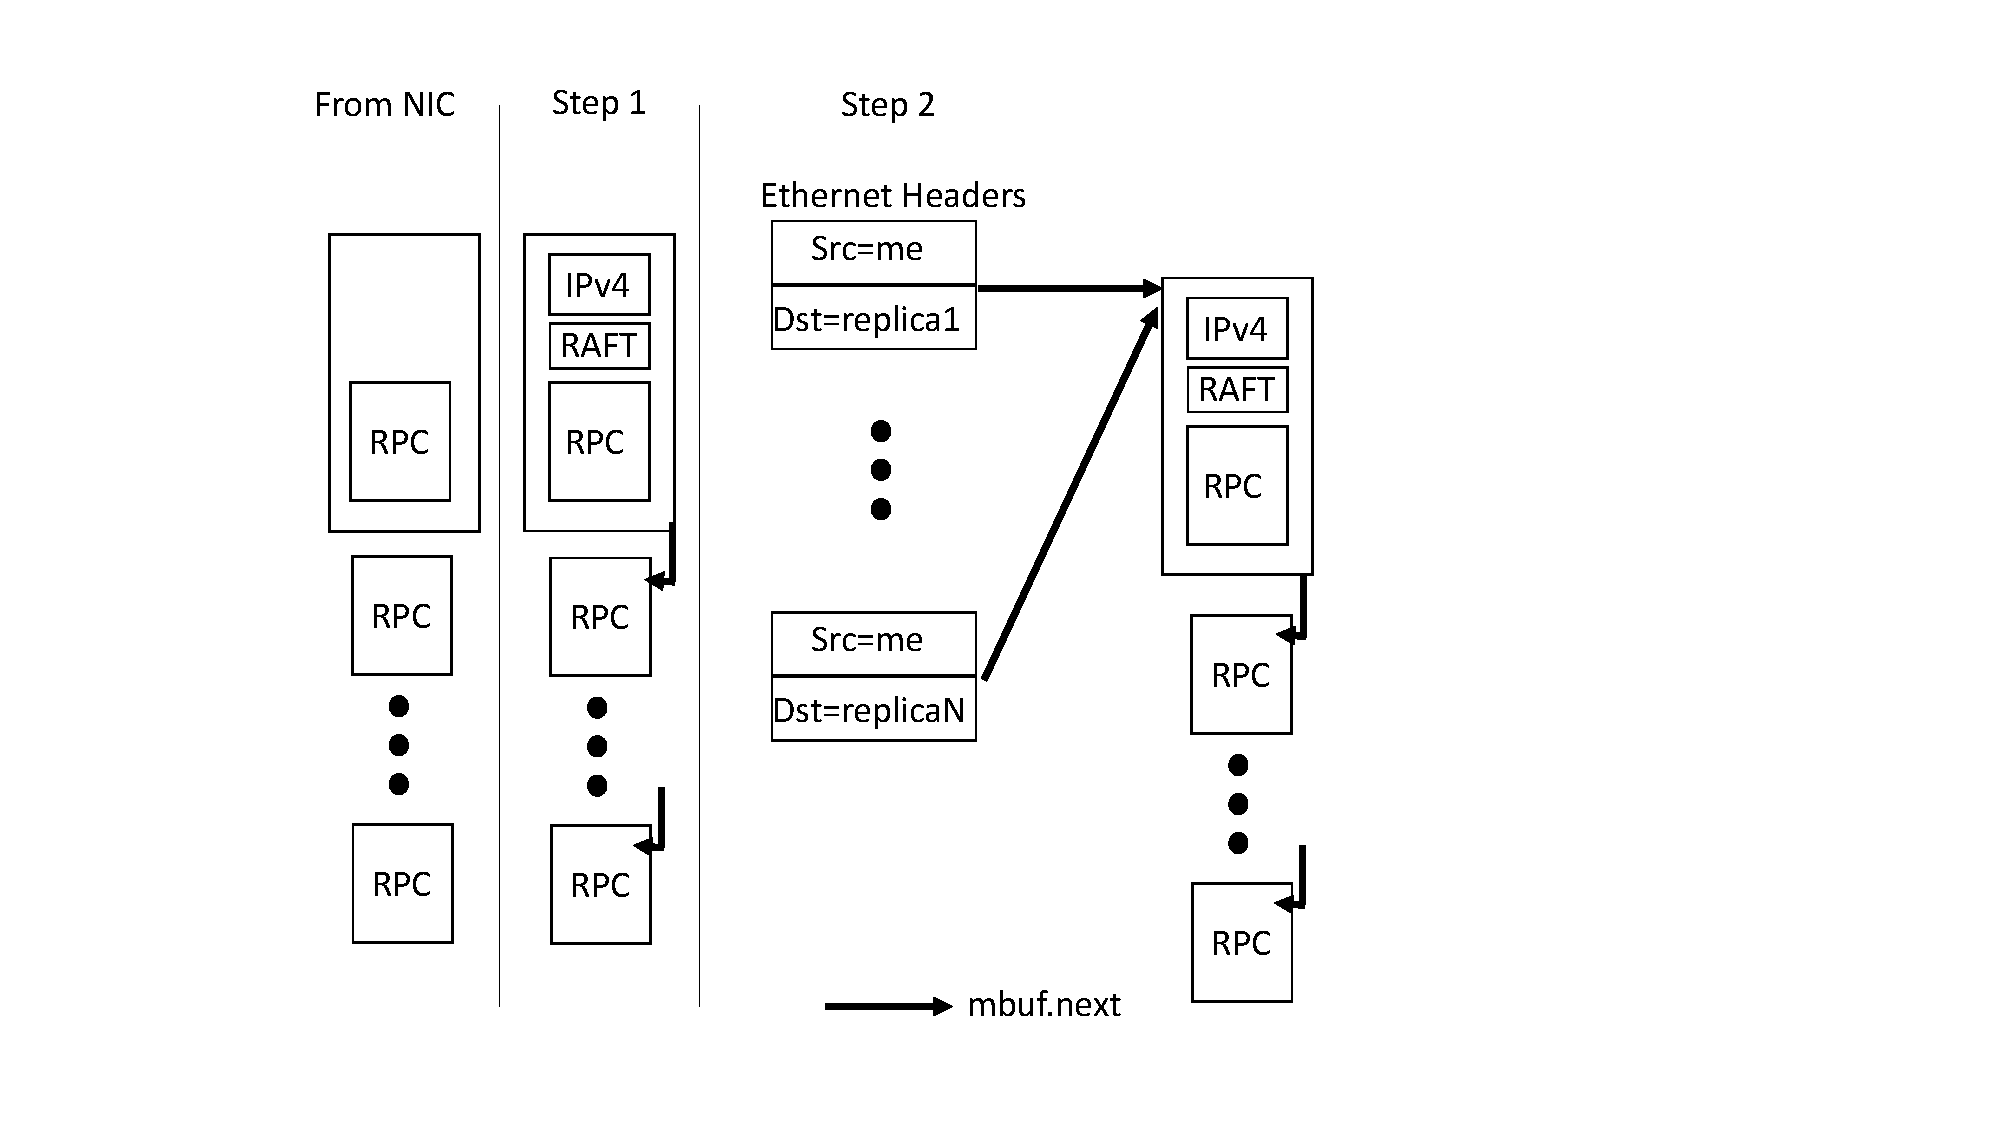
\includegraphics[width=0.7\textwidth,height=6cm]{figures/chain.pdf}
\caption{Zero Copy Batching}
\label{fig:zc_batch}
\end{figure}

This set of transformations to incoming request packets from clients at the
leader replica is summarized in Figure~\ref{fig:zc_batch}. 

\subsection{RPC Call Execution}
\label{sec:exec}
We now describe how RPC calls are executed and results returned to the
client. There are two important aspects of RPC call execution in Cyclone -
steering and at most once semantics.

An RPC call via Cyclone must traverse a specific RAFT core (and associated
consensus protocol instance) and specific application core. These details are
provided by the user when making the RPC call to the client side library
provided by Cyclone. The user therefore is aware of the number of execution
cores and RAFT instances and given complete control of \emph{RPC call steering}.
For most applications we envisage a simple modulo hashing scheme should suffice
for load balancing.

Cyclone provides at most once semantics. It supports a large but fixed (at
startup time) number of clients. Each RPC call from a client bears the client
number and a sequence number. \emph{Each execution core independently enforces
  execution of RPC calls in increasing sequence numbers}. This is done by
storing the last executed sequence number in a per-core durable datastructure as
part of the crash consistent transaction wrapping the execution of the RPC call
itself. Even in the presence of fail-overs, this durable memory of sequence
numbers seen from a client ensures at most once semantics. In addition to
guarding agains repeated execution of the same call, Cyclone also remembers the
\emph{results} of the last executed RPC call. This is done to assist clients
(particularly stateless clients). Cyclone allows the client to query the last
seen sequence number and result for that RPC call from the quorum of servers.

\section{A Durable Replicated Hash Table}
\label{sec:example}
We now demonstrate how Cyclone can be used in practice by putting together an
example of a linearizable hash table - a useful and common data structure.
[memcached]. The baseline is a durable hash table written in NVML that runs on a
single machine in client-server mode. The server side maintains the durable
open-addressed hash table and services client RPC calls to insert and delete
key-value pairs and lookup keys. Such a hash table is simple to derive from a
volatile hash table and readily available in NVML [nvml.io] as an example [src
  code link]. To use that (non client-server) example with Cyclone we added a
simple RPC call format, manually marshalled and demarshalled the few
arguments to the RPC call in an RPC call handler we wrote - a few tens of lines
of code. Finally, we added a simple client driver program (a few tens of
additional lines of code).

In order to use the hash table with Cyclone, we simply need to to declare the
RPC call handler as the point of entry to Cyclone at the server end.  The client
end issues RPC calls via Cyclone's client side library. Crucially neither side
involves fault awareness or fault recovery code - a key goal for Cyclone.

There are two interesting challenges in scaling the performance and improving
the utility of the linearizable and durable hash table. The first is to ensure
linearizability while scaling performance by adding RAFT cores and application
cores. The second is to support distributed transactions - that manipulate a set
of key-value pairs atomically in the face of failure.

\subsection{Scaling}
Scaling the performance of the hash table by using multiple RAFT cores and
application cores presents determinism related challenges. Two RPC calls being
steered through different RAFT cores can end up executing in different orders on
different replicas even if steered to the same application core. At the same time,
two RPC calls steered through the same RAFT core but dispatched to different
application cores can end up completing in different orders on different replicas.

Our solution to this problem in Cyclone is to observe that replicas of the hash
table require \emph{per-key determinism} and not determinism across \emph{all}
operations. We therefore steer operations to the same key to the same RAFT core
and the same application core, by hashing the key to determine the RAFT core and
execution core. The actual configuration of the hash table therefore can be
different across different replicas - for example due to the insertion of two
keys mapping to the same hash bucket completing in different orders across
different replicas. However, since the results of insert, delete and lookup
operations for a key depend only on previous operations to the same key the
replicas provide identical results for committed operations.

The RPC call steering mechanism described above leaves the programmer free to
use any synchronization mechanism they wish between concurrent accesses from the
application cores to the data structure, since the ordering between accesses
from different cores is allowed to be non-deterministic. For our open addressed
hash table we chose the simple scheme of a per-bucket lock.

\subsection{Distributed Transactions}
A useful primitive for many distributed systems is the ability to run
distributed transactions - an atomic sequence of conditional updates spanning
multiple machines. Distributed transactions have two distinct facets: atomicity
and fault tolerance. Distributed transactions appear atomic with respect to
other atomic transactions and simple updates or reads by virtue of standard
concurrency control techniques. A common technique is strict two phase
locking: acquire all locks, update the locked objects and finally release all
the locks. We believe that NVM application programmers - particularly those
having experience with concurrent code should not find it hard to deal with
distributed concurrency. The hard part for most programmers is likely to be the
second aspect: fault tolerance. A distributed transaction spans many machines
and has a large footprint to clean up in the event of failure. Failure handling
is made more complex when considering cascading failures - further failures
while recovering from a failure. Cyclone was designed to allow primitives such
as distributed transctions to be added without the programmer needing to worry
about faults or write fault recovery code. As an exercise we show how to add
support for distributed transactions to our hash table.

We support distributed transactions in our hash table by allowing the user to
specify a group of insert/delete/lookup operations that must occur
atomically. We use the existing bucket locks to implement a simple two phase
locking protocol to implement the transction. A client makes an RPC call to the
server specifying the transaction and the server executes it on the client's
behalf. Execution of the transaction has four distinct phases: acquire locks,
verify values, apply updates and finally release locks.

We guard against faults by executing the RPC call on a quorum of
machines via Cyclone. Since execution of the RPC call leaves \emph{externally
  visible side effects} by virtue of the RPC calls it makes we require output
commit [] - the property that the execution is guaranteed to complete once it
starts. This is simply achieved by a flag in the RPC call that turns off
decoupled execution (Section~\ref{sec:decouple}). The flag causes execution to
start only after the RPC call has been successfully replicated.

Next, we need to ensure that although every machine in the quorum makes all
necessary RPC calls, the call itself is executed only once. This is achieved by
using Cyclone's at most once semantics. All machines in the quorum executing the
transaction use the same client identifier and the same montonically increasing
sequence of RPC call numbers. Finally, we need to deal with the fact that
Cyclone only remembers the last executed RPC call for a client. This means that
if different machines in the quorum move at different speeds, some machines will
not receive a response to the RPC call - they will instead receive an error that
tells them that they are too far behind.

To ensure that the transaction is still guaranteed to complete, we use a
\emph{different} client identifier for each phase. Thus, until the transaction
completes and a new one is started the response for any RPC call continues to be
available. Figure~\ref{fig:dist_tx} shows in pseudocode the server side details
of a transaction. One initiated, the distributed transaction is guaranteed to
complete given quorum availabilty. However, if the client requires intimation of
completion, the final transaction state can be written to a distinguished
partition as part of the transaction itself.

We note that this design is not intended for performance, under the assumption
that distributed transactions will be infrequent compared to single key
operations.  On the other hand, it is worth comparing the lack of any need for
explicit fault recovery in Cyclone with fault recovery in systems systems that
explicity require such cleanup [FARM, also refer to pages].  We believe that
such designs, which make availability easy for NVM applications are key to
increasing the adoption rate of NVM by data center operators.

\begin{figure}
{ \scriptsize
\begin{verbatim}
wait until RPC call is replicated
respond to client saying tx accepted for execution
acquire:
 set client identifier to 1
 for each machine
   Acquire write or read locks on the machine
   If machine reponds RPC sequence too old
     Transaction completed by someone else

update:
 set client identifier to 2
 for each machine
   Update object
   If machine reponds RPC sequence too old
     Transaction completed by someone else
 
release:
 set client identifier to 3
 for each machine
   Update object
   If machine reponds RPC sequence too old
     Transaction completed by someone else

optional:
 write transaction result to <quorum_tx_result>
\end{verbatim}
}
\caption{Distributed Transactions}
\label{fig:dist_tx}
\end{figure}

\section{Evaluation}

\begin{figure*}
\begin{tabular}{cc}
\begin{minipage}{0.5\textwidth}
  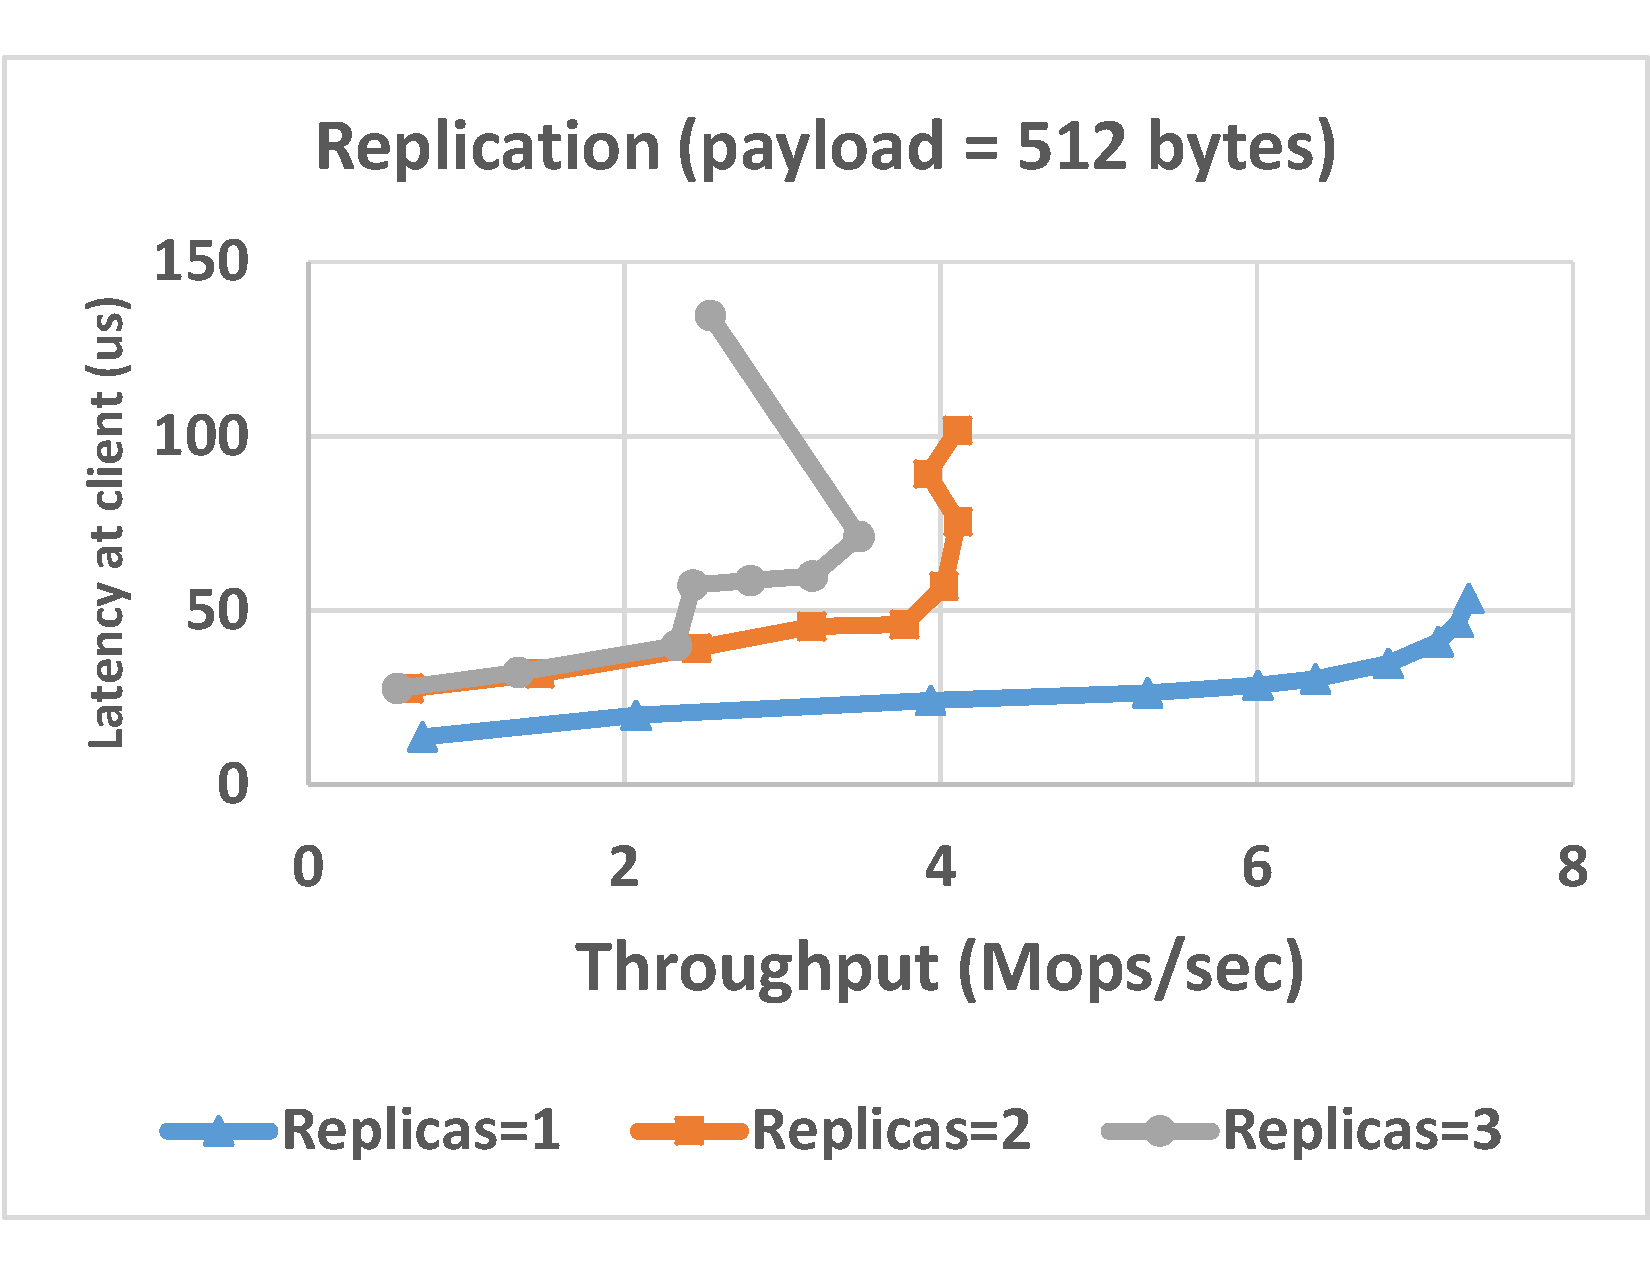
\includegraphics[width=\textwidth,height=6cm]{results/replication_mops_0.pdf}
\end{minipage}&
\begin{minipage}{0.5\textwidth}
  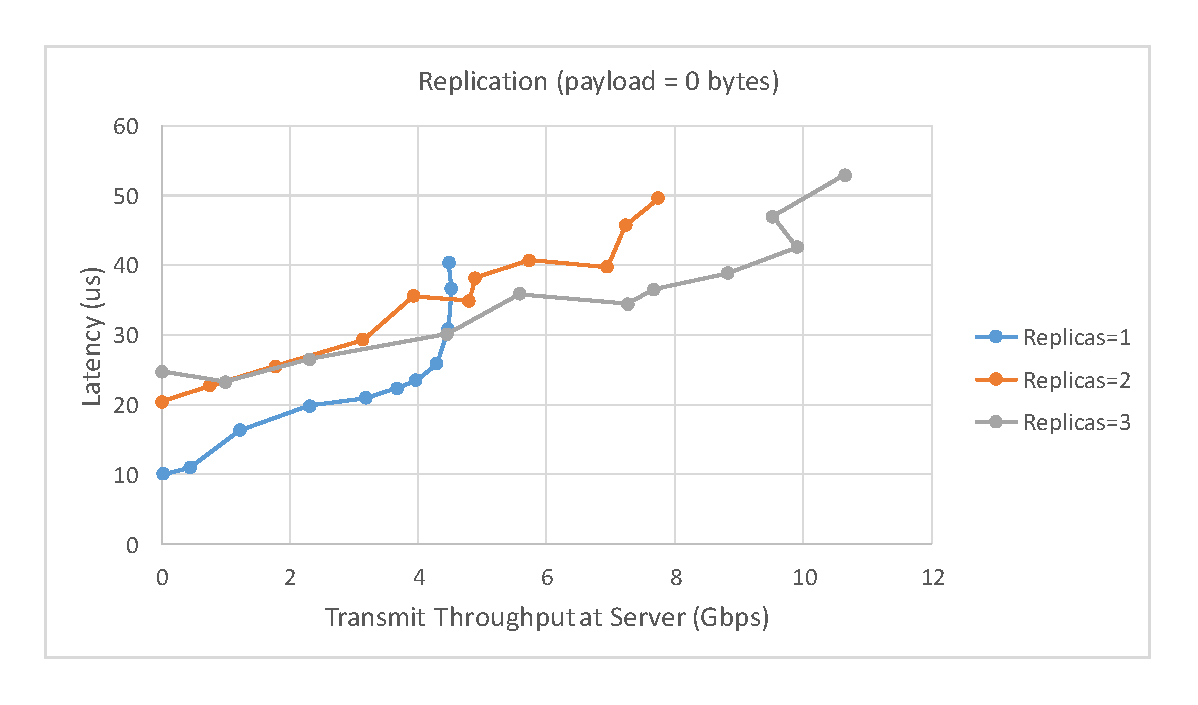
\includegraphics[width=\textwidth,height=6cm]{results/replication_gbps_0.pdf}
\end{minipage}\\
\begin{minipage}{0.5\textwidth}
  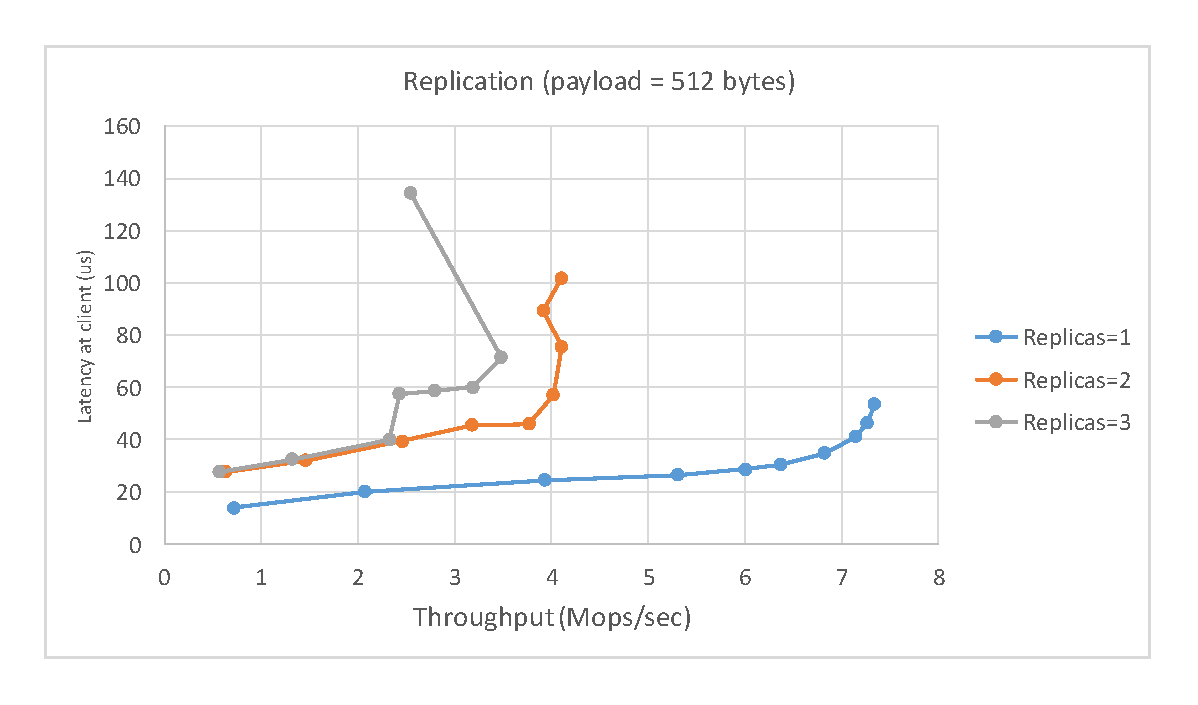
\includegraphics[width=\textwidth,height=6cm]{results/replication_mops_512.pdf}
\end{minipage}&
\begin{minipage}{0.5\textwidth}
  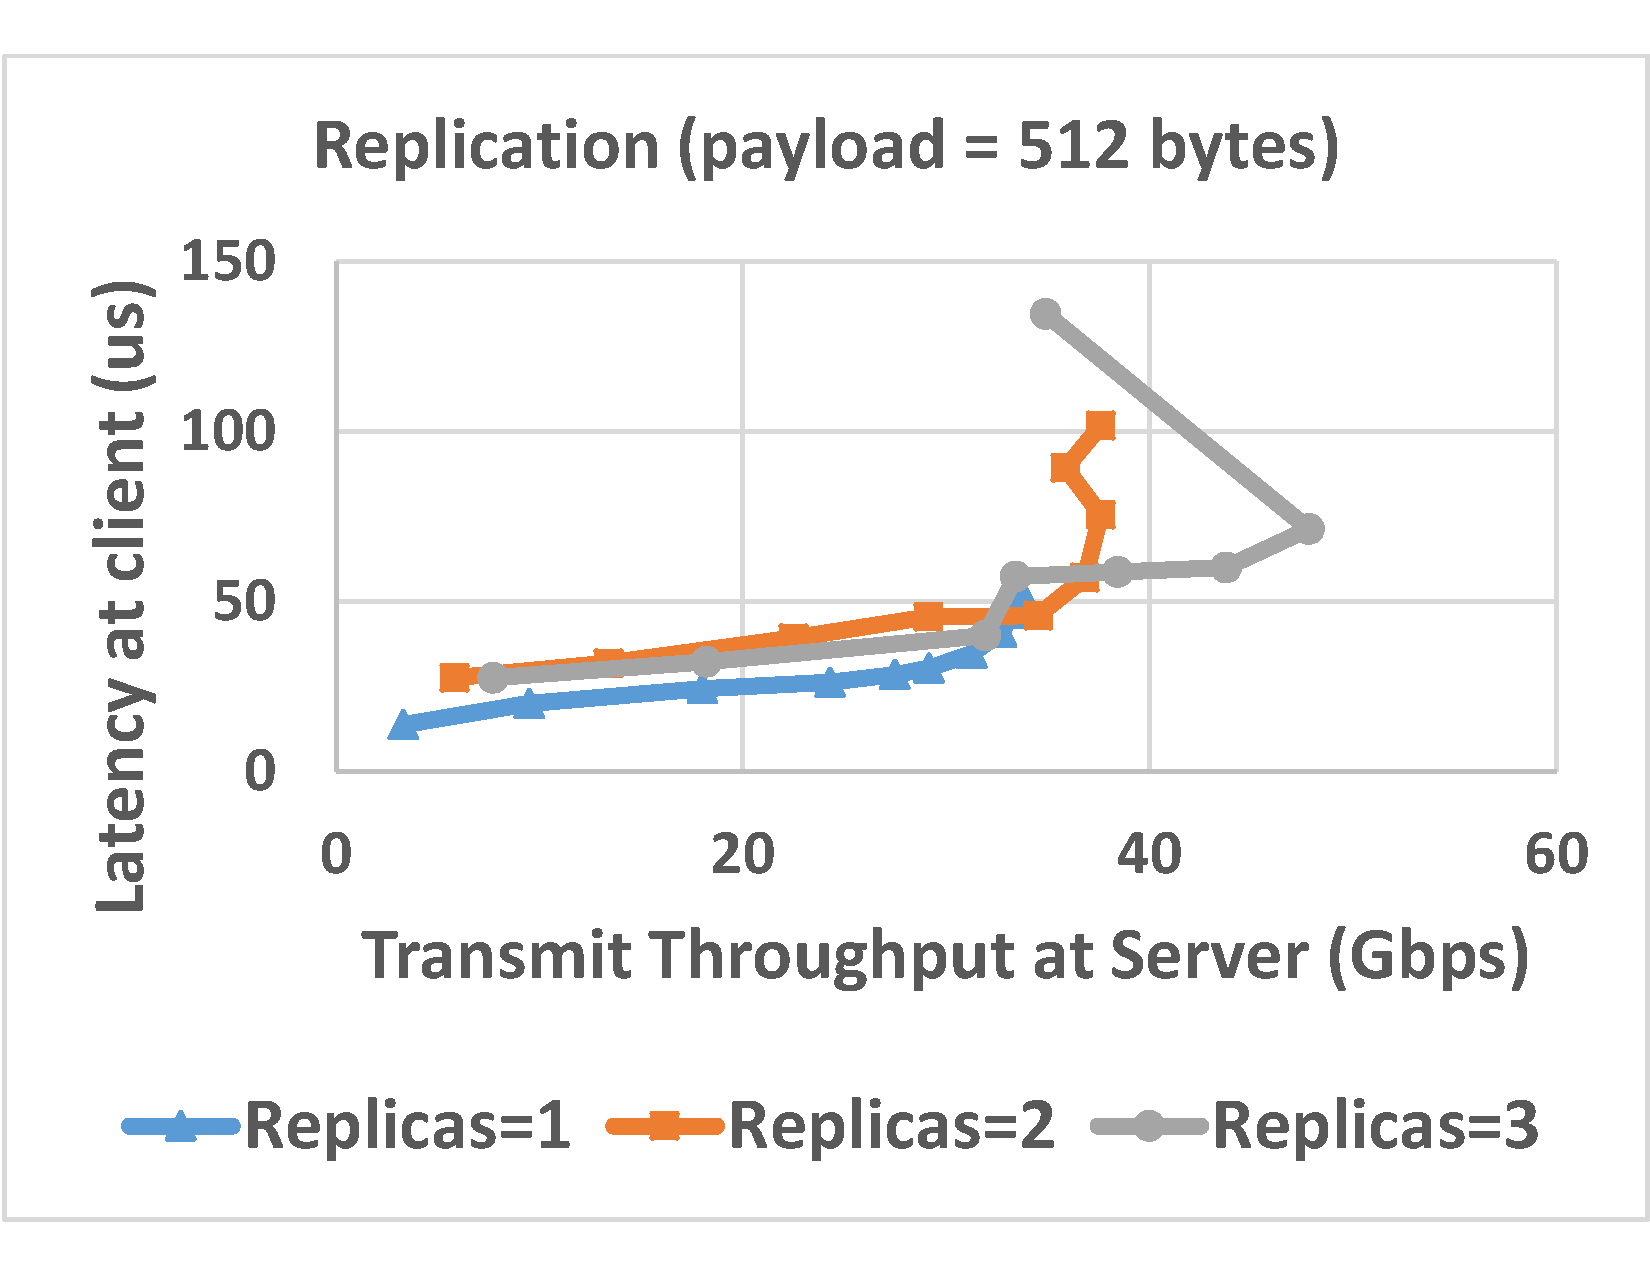
\includegraphics[width=\textwidth,height=6cm]{results/replication_gbps_512.pdf}
\end{minipage}
\end{tabular}
\caption{Pure Replication}
\label{fig:pure_rep}
\end{figure*}

\begin{figure}
  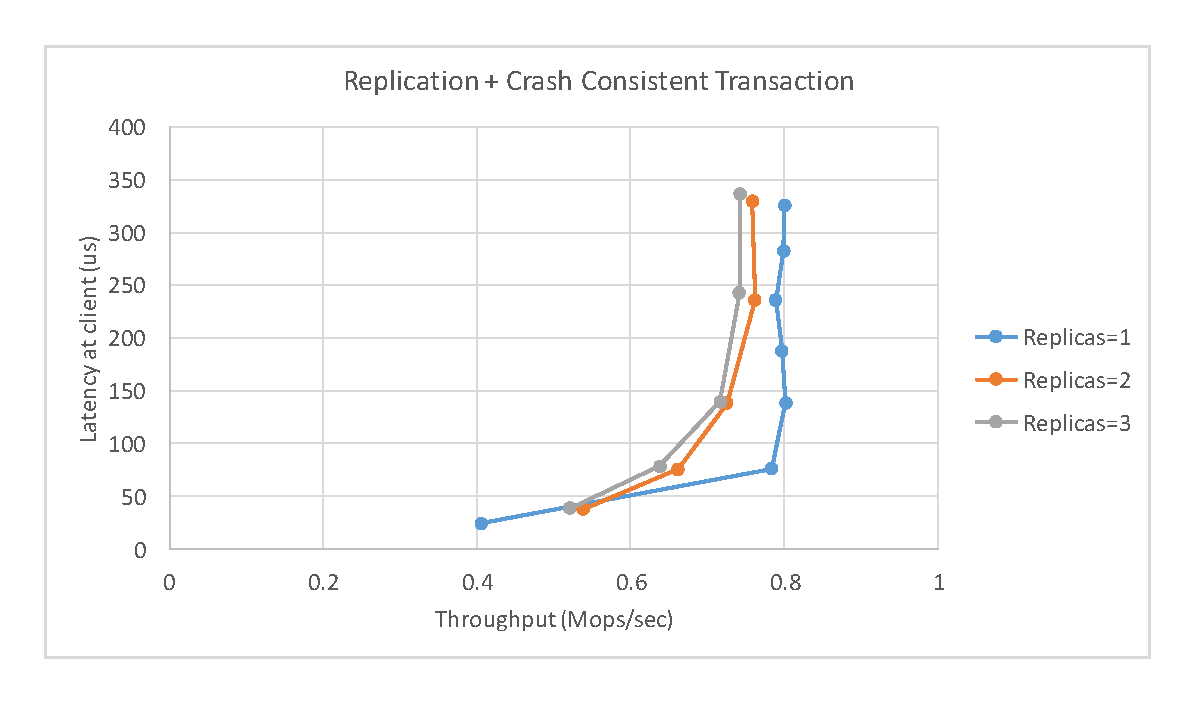
\includegraphics[width=0.5\textwidth,height=6cm]{results/cc_mops.pdf}
  \caption{Crash Consistency + Replication}
  \label{fig:cc_rep}
\end{figure}

\begin{figure}
  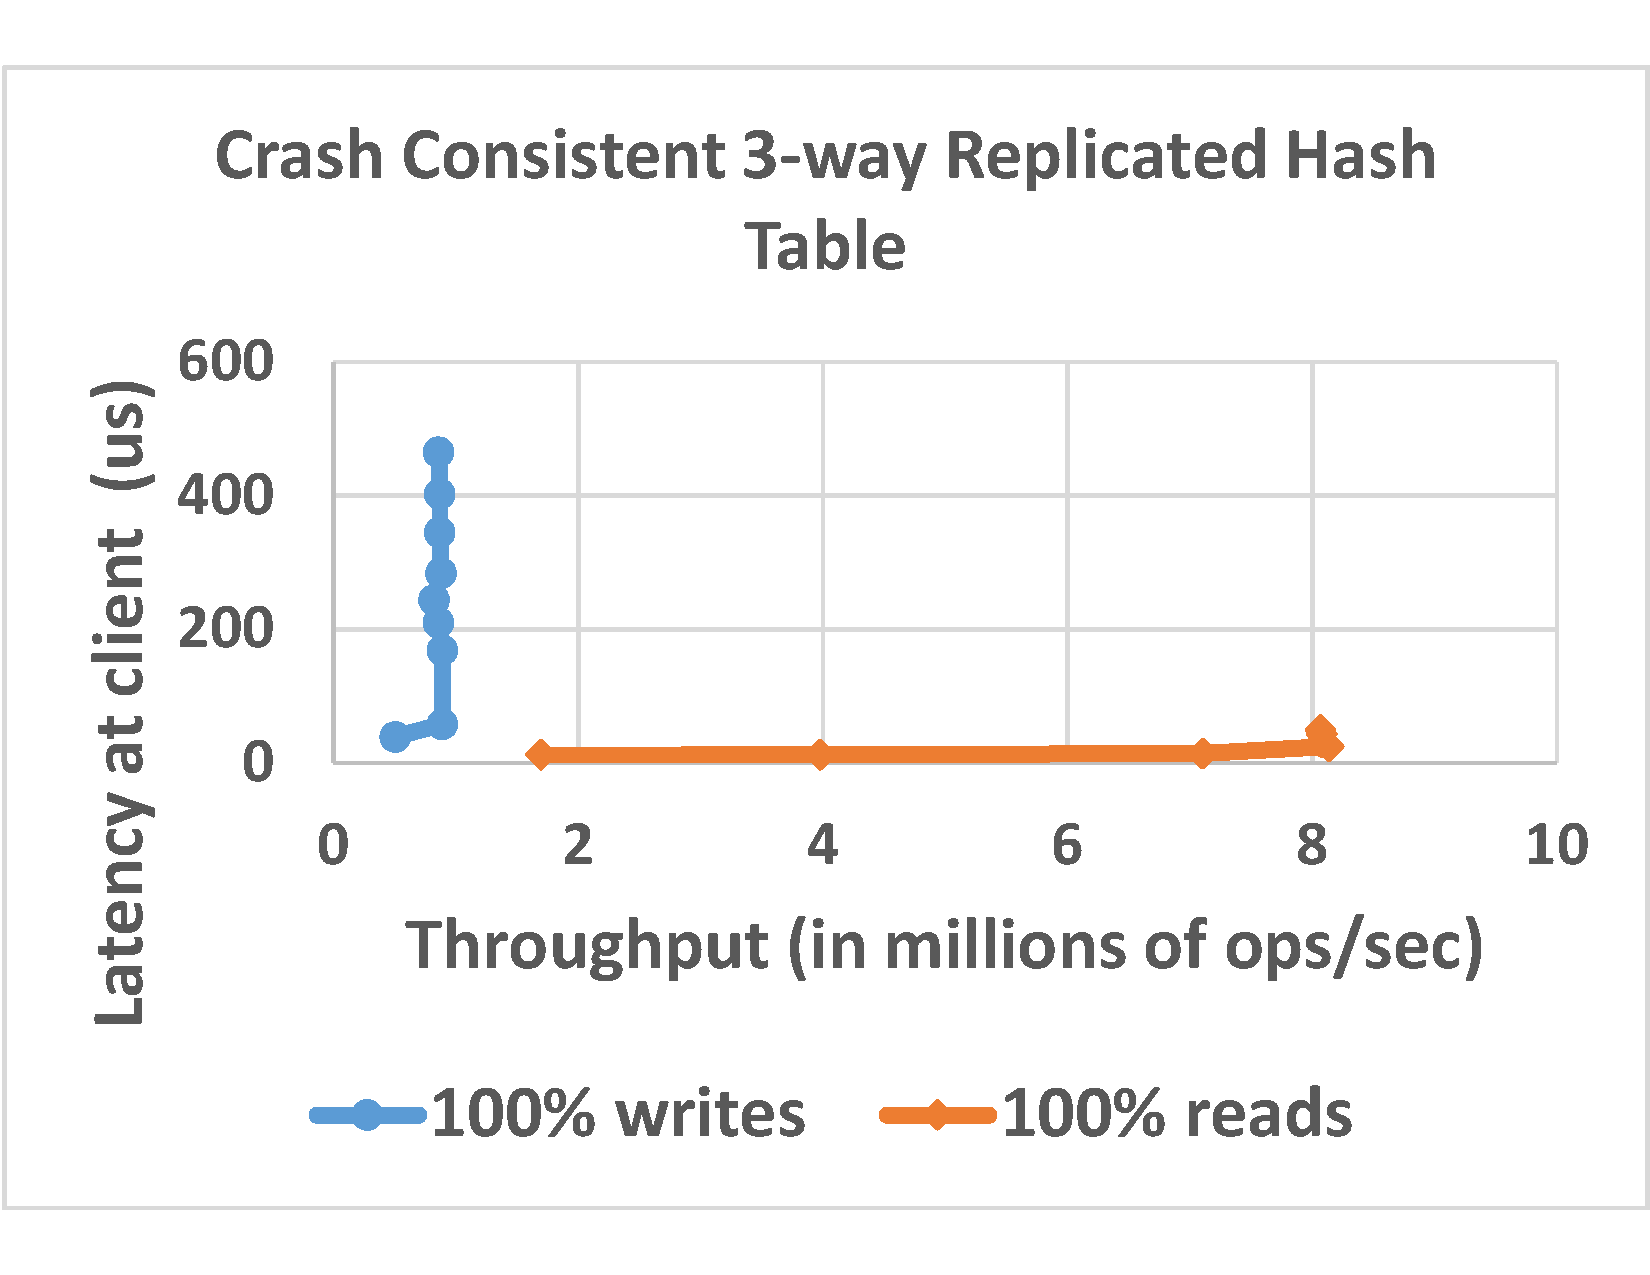
\includegraphics[width=0.5\textwidth,height=6cm]{results/app_mops.pdf}
  \caption{Crash Consistent Replicated Hash Table}
  \label{fig:app_rep}
\end{figure}

\section{Conclusion}

\end{document}



